\documentclass{article}
\usepackage[top=0.5in, bottom=0.5in, left=1.25in, right=1.25in]{geometry}

\usepackage{amsmath, array, enumerate, sfmath, pgfplots, pgfplotstable, tcolorbox, graphicx, color, colortbl}
\pgfplotsset{compat = newest}
\usepgfplotslibrary{statistics}
\usetikzlibrary{arrows.meta}
\renewcommand{\familydefault}{\sfdefault}
\raggedright
\pagestyle{empty}

\newcounter{example}[section]
\newenvironment{example}[1][]{\refstepcounter{example}\par\medskip
   {\color{red}\textbf{Example~\theexample. #1}}}{\medskip}

\begin{document}

\section*{Scatterplots and Correlation}

\begin{tcolorbox}[colframe=orange!70!white, coltitle=black, title=\textbf{Summary}]
\begin{enumerate}
    \item Scatterplots are data displays that is simply plotting points.
    \item Correlation means that the data points tend upwards or downwards, or possibly neither.
\end{enumerate}
\end{tcolorbox}
\vspace{0.75in}

\subsection*{Scatterplots}

\vspace{0.25in}

\begin{tcolorbox}[colframe=green!20!black, colback = green!30!white,title=\textbf{Scatterplot}]
A \textbf{scatterplot} is a visual display which can be used to examine an association between two variables, usually $x$ and $y$.
\end{tcolorbox}
\vspace{0.5in}

\begin{itemize}
    \item The independent variable, $x$, is called the {\color{blue}\textbf{explanatory variable}}.
    \item The dependent variable, $y$, is called the {\color{blue}\textbf{response variable}}.
    \item Scatterplots allow us to see if there is a relationship between the two variables.
\end{itemize}
\vspace{1.5in}


\begin{example}
The table below shows the age of a certain model of car (in years) with the cars current value (in thousands of dollars). Create a scatterplot for the data.	\newline\\
\begin{minipage}{0.3\textwidth}
\begin{tabular}{c|c}
\textbf{Age} & \textbf{Value} \\ \hline
2 & 15 	\\
3 & 12	\\
3 & 13	\\
2 & 14	\\
4 & 13	\\
5 & 10	\\
6 & 10.5	\\
1 & 16.5	\\
0 & 18		\\
4 & 14		\\
7 & 11		
\end{tabular}
\end{minipage}
\hspace{0.25cm}
\begin{minipage}{0.6\textwidth}
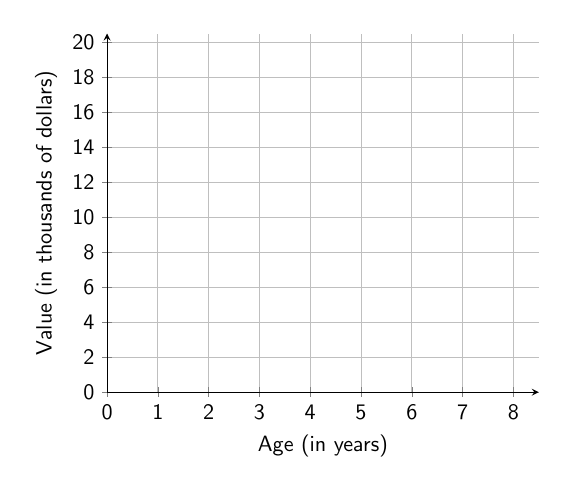
\begin{tikzpicture}[scale=0.8]
	\begin{axis}[
	axis lines = left, grid,
	xlabel = {Age (in years)},
	ylabel = {Value (in thousands of dollars)},
	xmin = 0, xmax = 8.5,
	ymin = 0, ymax = 20.5,
	xtick = {0,1,...,8},
	ytick = {0,2,...,20}
	]
	\end{axis}
\end{tikzpicture}
\end{minipage}
\end{example}

\newpage 

\subsection*{Correlation}

Often times, the data in a scatterplot has some pattern to it. \newline\\	

\begin{tcolorbox}[colframe=green!20!black, colback = green!30!white,title=\textbf{Correlation}]
A \textbf{correlation} between two variables examines how the response variable's ($y$) values change as the explanatory variable's ($x$) values change.
\end{tcolorbox}

\vspace{0.5in}

There are 3 correlation types: positive, negative, and none (a.k.a. no correlation)
\vspace{0.25in}

\begin{center}
\begin{tabular}{ccc}
    Positive Correlation & Negative Correlation & No Correlation    \\
    As $x$ increases, so does $y$ & As $x$ increases, $y$ decreases & No visible patter between $x$ and $y$ \\[10pt]
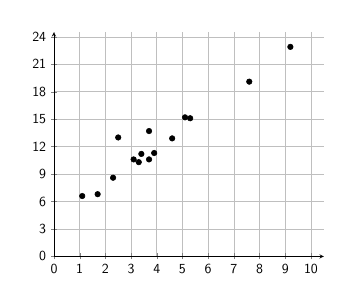
\begin{tikzpicture}[scale=0.5]
	\begin{axis}[
	axis lines = left, grid,
	xmin = 0, xmax = 10.5,
	ymin = 0, ymax = 24.5,
	xtick = {0,1,...,10},
	ytick = {0,3,...,24}
	]
    \addplot [only marks] coordinates {
    (7.6, 19.1)
    (9.2, 22.9)
    (3.3, 10.3)
    (1.1, 6.6)
    (3.7, 10.6)
    (3.9, 11.3)
    (4.6, 12.9)
    (2.3, 8.6)
    (5.1, 15.2)
    (5.3, 15.1)
    (2.5, 13)
    (3.4, 11.2)
    (3.1, 10.6)
    (1.7, 6.8)
    (3.7, 13.7)
    };
    \end{axis}
\end{tikzpicture}
&
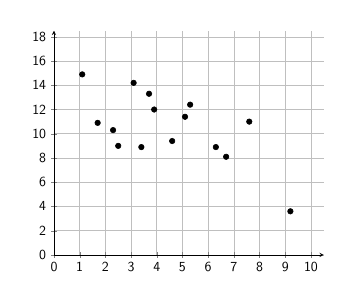
\begin{tikzpicture}[scale=0.5]
	\begin{axis}[
	axis lines = left, grid,
	xmin = 0, xmax = 10.5,
	ymin = 0, ymax = 18.5,
	xtick = {0,1,...,10},
	ytick = {0,2,...,18}
	]
    \addplot [only marks] coordinates{
    (7.6, 11.0)
    (9.2, 3.6)
    (6.3, 8.9)
    (1.1, 14.9)
    (6.7, 8.1)
    (3.9, 12.0)
    (4.6, 9.4)
    (2.3, 10.3)
    (5.1, 11.4)
    (5.3, 12.4)
    (2.5, 9.0)
    (3.4, 8.9)
    (3.1, 14.2)
    (1.7, 10.9)
    (3.7, 13.3)
    };
    \end{axis}
\end{tikzpicture}
&
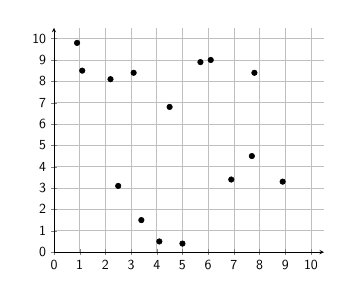
\begin{tikzpicture}[scale=0.5]
	\begin{axis}[
	axis lines = left, grid,
	xmin = 0, xmax = 10.5,
	ymin = 0, ymax = 10.5,
	xtick = {0,1,...,10},
	ytick = {0,1,...,10}
	]
    \addplot [only marks] coordinates{
    (6.9, 3.4)
    (7.7, 4.5)
    (0.9, 9.8)
    (3.4, 1.5)
    (8.9, 3.3)
    (5.7, 8.9)
    (3.1, 8.4)
    (2.2, 8.1)
    (4.5, 6.8)
    (4.1, 0.5)
    (5.0, 0.4)
    (7.8, 8.4)
    (2.5, 3.1)
    (6.1, 9.0)
    (1.1, 8.5)
    };
    \end{axis}
\end{tikzpicture}
\end{tabular}
\end{center}

\vfill

\begin{center}
\textsc{Means of $x$- and $y$-coordinates in red; along with count of points.} \newline\\
\begin{tabular}{ccc}
    Positive Correlation & Negative Correlation & No Correlation    \\
    More points in Quads 1 and 3 & 
    More points in Quads 2 and 4 &
    Just about same number of points in each \\[10pt]
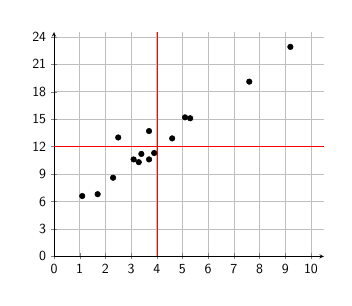
\begin{tikzpicture}[scale=0.5]
	\begin{axis}[
	axis lines = left, grid,
	xmin = 0, xmax = 10.5,
	ymin = 0, ymax = 24.5,
	xtick = {0,1,...,10},
	ytick = {0,3,...,24}
	]
    \addplot [only marks] coordinates {
    (7.6, 19.1)
    (9.2, 22.9)
    (3.3, 10.3)
    (1.1, 6.6)
    (3.7, 10.6)
    (3.9, 11.3)
    (4.6, 12.9)
    (2.3, 8.6)
    (5.1, 15.2)
    (5.3, 15.1)
    (2.5, 13)
    (3.4, 11.2)
    (3.1, 10.6)
    (1.7, 6.8)
    (3.7, 13.7)
    };
    \draw [color=red] (axis cs: 4.03,24.5) -- (4.03,0);
    \draw [color=red] (axis cs: 10.5,12.09) -- (0,12.09);
    \end{axis}
\end{tikzpicture}
&
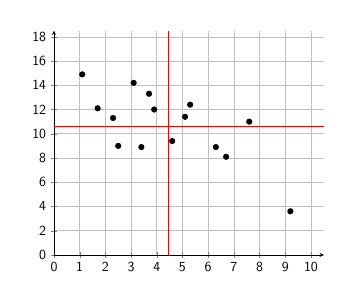
\begin{tikzpicture}[scale=0.5]
	\begin{axis}[
	axis lines = left, grid,
	xmin = 0, xmax = 10.5,
	ymin = 0, ymax = 18.5,
	xtick = {0,1,...,10},
	ytick = {0,2,...,18}
	]
    \addplot [only marks] coordinates{
    (7.6, 11.0)
    (9.2, 3.6)
    (6.3, 8.9)
    (1.1, 14.9)
    (6.7, 8.1)
    (3.9, 12.0)
    (4.6, 9.4)
    (2.3, 11.3)
    (5.1, 11.4)
    (5.3, 12.4)
    (2.5, 9.0)
    (3.4, 8.9)
    (3.1, 14.2)
    (1.7, 12.1)
    (3.7, 13.3)
    };
    \draw [color=red] (axis cs: 4.43,0) -- (axis cs: 4.43,18.5);
    \draw [color=red] (axis cs: 0,10.6) -- (axis cs: 10.5,10.6);
    \end{axis}
\end{tikzpicture}
&
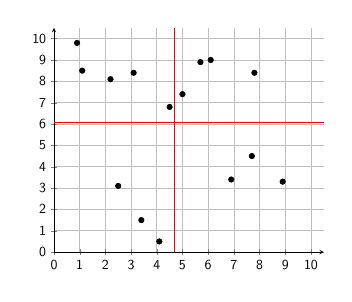
\begin{tikzpicture}[scale=0.5]
	\begin{axis}[
	axis lines = left, grid,
	xmin = 0, xmax = 10.5,
	ymin = 0, ymax = 10.5,
	xtick = {0,1,...,10},
	ytick = {0,1,...,10}
	]
    \addplot [only marks] coordinates{
    (6.9, 3.4)
    (7.7, 4.5)
    (0.9, 9.8)
    (3.4, 1.5)
    (8.9, 3.3)
    (5.7, 8.9)
    (3.1, 8.4)
    (2.2, 8.1)
    (4.5, 6.8)
    (4.1, 0.5)
    (5.0, 7.4)
    (7.8, 8.4)
    (2.5, 3.1)
    (6.1, 9.0)
    (1.1, 8.5)
    };
    \draw [color=red] (axis cs: 4.7,0) -- (axis cs: 4.7,10.5);
    \draw [color=red] (axis cs: 0,6.1) -- (axis cs: 10.5,6.1);
    \end{axis}
\end{tikzpicture}
\end{tabular}
\end{center}

\vfill 

\newpage 

\subsubsection*{Correlation vs. Causation}
\vspace{0.5in}

\begin{center}
\fbox{\parbox{5.25in}{
\begin{center}
\begin{Large}
{\color{red}\textbf{*** VERY IMPORTANT ***}}
\end{Large}

Just because there may be a strong correlation (an {\color{blue}\textbf{association}}) between two variables \\ \textbf{DOES NOT MEAN THAT ONE CAUSES THE OTHER TO HAPPEN.}
\end{center}}}
\end{center}

\vspace{1in}

For instance, dogs with larger paws tend to have larger weights, but we can not conclude that large paws cause a large weight.
\vspace{0.5in}

If there is a strong correlation, there may be lurking variable(2) and/or confounding at play.

\vspace{0.5in}

\begin{tcolorbox}[colframe=green!20!black, colback = green!30!white,title=\textbf{Lurking Variable}]
A \textbf{lurking variable} is an explanatory variable that has an influence in the outcome of a study or experiment but is not considered in the study or experiment.
\end{tcolorbox}

\vspace{1in}

\begin{tcolorbox}[colframe=green!20!black, colback = green!30!white,title=\textbf{Confounding}]
\textbf{Confounding} occurs when we can not distinguish the effect(s) one (or many) explanatory has (have) on a response variable.
\end{tcolorbox}



\end{document}
